\documentclass[tikz,border=0mm]{standalone}
\usepackage[utf8]{vietnam}
\usetikzlibrary{positioning,calc,arrows,arrows.meta}
\begin{document}
	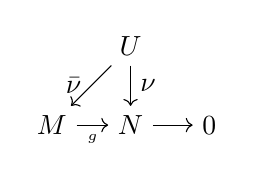
\begin{tikzpicture}
		\node (N) at (0,0){$N$};
		\node[above of=N] (U){$U$};
		\node[right of=N] (O){$0$};
		\node[left of=N] (M){$M$};
		\draw[->] (U)--(N) node[midway,right]{$\nu$};
		\draw[->] (U)--(M) node[midway,left]{$\bar\nu$};
		\draw[->] (M)--(N) node[midway,below]{\tiny $g$};
		\draw[->] (N)--(O);
	\end{tikzpicture}
	% khác biệt giữa 
	% above =of N (khoảng cách lớn hơn)
	% và above of= N
	% https://tex.stackexchange.com/.../difference-between...
	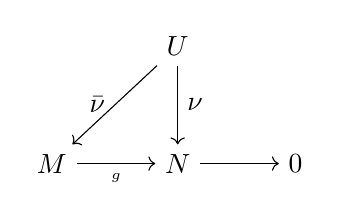
\begin{tikzpicture}
		\node (N) at (0,0){$N$};
		\node[above =of N] (U){$U$};
		\node[right =of N] (O){$0$};
		\node[left =of N] (M){$M$};
		\draw[->] (U)--(N) node[midway,right]{$\nu$};
		\draw[->] (U)--(M) node[midway,left]{$\bar\nu$};
		\draw[->] (M)--(N) node[midway,below]{\tiny $g$};
		\draw[->] (N)--(O);
	\end{tikzpicture}
	% TikZ manual page 252
	% edge cũng tiện
	% Tuy nhiên hoàn toàn có thể dùng \draw 
	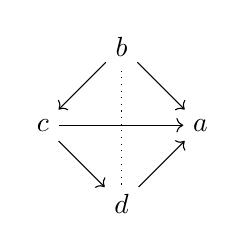
\begin{tikzpicture}
		\node (a) at (0:1) {$a$};
		\node (b) at (90:1) {$b$}  edge [->] (a);
		\node (c) at (180:1) {$c$} edge [->] (a) 
		edge [<-] (b);
		\node (d) at (270:1) {$d$} edge [->] (a)
		edge [dotted] (b)
		edge [<-] (c);
	\end{tikzpicture}
	% TikZ manual page 252
	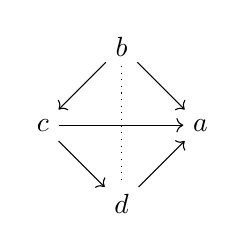
\begin{tikzpicture}
		\node foreach \name/\angle in {a/0,b/90,c/180,d/270}
		(\name) at (\angle:1) {$\name$};
		\path[->] (b) edge (a)
		edge (c)
		edge [-,dotted] (d)
		(c) edge (a)
		edge (d)
		(d) edge (a);
	\end{tikzpicture}
	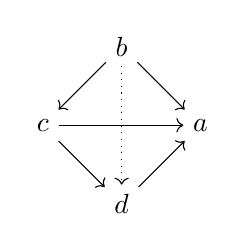
\begin{tikzpicture}
		\node (a) at (0:1) {$a$};
		\node (b) at (90:1) {$b$};
		\node (c) at (180:1) {$c$};
		\node (d) at (270:1) {$d$};
		\draw[->] (b)--(a);
		\draw[->] (b)--(c);
		\draw[->] (c)--(d);
		\draw[->] (c)--(a);
		\draw[->] (d)--(a);
		\draw[->,dotted] (b)--(d);
	\end{tikzpicture}
	%https://tex.stackexchange.com/.../how-to-draw-multiple...
	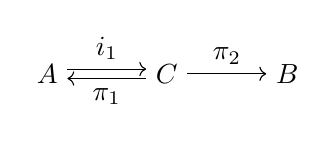
\begin{tikzpicture}
		\node (C) at (0,0){$C$};
		\node[right =of C] (B){$B$};
		\node[left =of C] (A){$A$};
		\draw[->] ($(A.east)+(0,.6mm)$)--($(C.west)+(0,.6mm)$) node[midway,above]{$i_1$};
		\draw[<-] ($(A.east)+(0,-.6mm)$)--($(C.west)+(0,-.6mm)$) node[midway,below]{$\pi_1$};
		\draw[->] (C)--(B) node[midway,above]{$\pi_2$};
	\end{tikzpicture}
	% Cách 2: ko dùng calc, mà dùng yshift (hay hơn)
	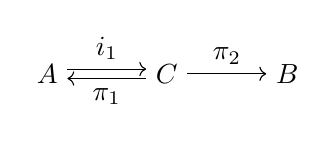
\begin{tikzpicture}
		\node (C) at (0,0){$C$};
		\node[right =of C] (B){$B$};
		\node[left =of C] (A){$A$};
		\draw[->] ([yshift=.6mm]A.east)--([yshift=.6mm]C.west) node[midway,above]{$i_1$};
		\draw[<-] ([yshift=-.6mm]A.east)--([yshift=-.6mm]C.west) node[midway,below]{$\pi_1$};
		\draw[->] (C)--(B) node[midway,above]{$\pi_2$};
	\end{tikzpicture}
	%https://tex.stackexchange.com/.../co-equalizer-diagram-in...
	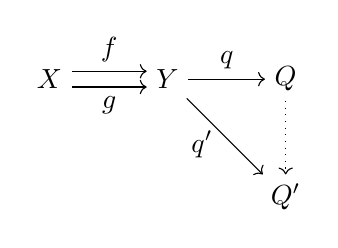
\begin{tikzpicture}[node distance=1.5cm]
		\node (Y) at (0,0){$Y$};
		\node[right of=Y] (Q){$Q$};
		\node[left of=Y] (X){$X$};
		\node[below of=Q] (Q'){$Q'$};
		\draw[->] ([yshift=1mm]X.east)--([yshift=1mm]Y.west) node[midway,above]{$f$};
		\draw[->] ([yshift=-1mm]X.east)--([yshift=-1mm]Y.west) node[midway,below]{$g$};
		\draw[->,dotted] (Q)--(Q');
		\draw[->] (Y)--(Q) node[midway,above]{$q$};
		\draw[->] (Y)--(Q') node[pos=.2,below=1mm]{$q'$};
	\end{tikzpicture}
	\begin{tikzpicture}[node distance=2cm]
		\node (A) at (0,0){$A$};
		\node[right of=A] (B){$B$};
		\node[below of=A] (C){$C$};
		\node[below of=B] (D){$D$};
		\draw[->] (A)--(B) node[midway,above]{$f$};
		\draw[->] (B)--(D) node[midway,right]{$h$};
		\draw[->] (A)--(C) node[midway,left]{$h$};
		\draw[->] (C)--(D) node[midway,below]{$g$};
		\draw (current bounding box.east) 
		node[right=.5cm,fill=blue!20]{$h\circ f=g\circ h$};
		\draw (current bounding box.north) node[above]
		{Sự tương đương tô-pô của các đồng phôi.};
	\end{tikzpicture}
	\begin{tikzpicture}
		\node (G) at (0,0){$G$};
		\node[right of=G,node distance=2.5cm] (H){$H$};
		\node[below of=G,node distance=1.5cm] (Gker){$G/{\rm ker}(f)$};
		\draw[->] (G)--(H) node[midway,above]{$f$};
		\draw[->] (G)--(Gker) node[midway,left]{$\pi$};
		\draw[->,dashed] (Gker)--(H) node[midway,below right]{$\tilde{f}$};
		\draw (current bounding box.north) node[above]
		{Định lý đồng cấu thứ nhất.};
	\end{tikzpicture}
	% https://en.wikipedia.org/wiki/Commutative_diagram
	% chưa ưng ý lắm
	% có thể đặt node trên đường cong như thế nào?
	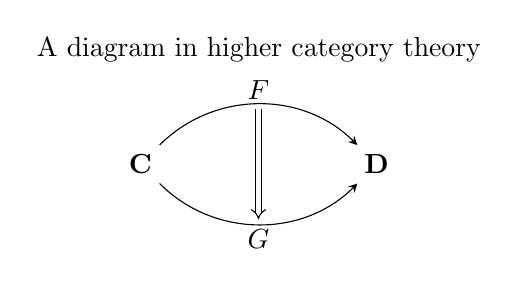
\begin{tikzpicture}
		\def\a{1.5}
		\node (C) at (-\a,0){$\mathbf{C}$};
		\node (D) at (\a,0){$\mathbf{D}$};
		\draw[-stealth] (C) to[out=45,in=135] (D) node[midway,above=7mm](F){$F$};
		\draw[-stealth] (C) to[out=-45,in=-135] (D) node[midway,below=7mm](G){$G$};
		\draw[double equal sign distance, -Implies] (F)--(G);
		\draw (current bounding box.north) node[above]
		{A diagram in higher category theory};
	\end{tikzpicture}
	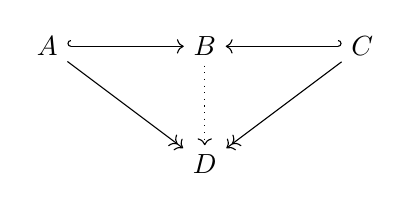
\begin{tikzpicture}[node distance=2cm]
		\node (B) at (0,0){$B$};
		\node[right of=B] (C){$C$};
		\node[left of=B] (A){$A$};
		\node[below of=B,node distance=1.5cm] (D){$D$};
		\draw[->,dotted] (B)--(D);
		\draw[<-{Hooks[right]}] (B)--(A);
		\draw[<-{Hooks[left]}] (B)--(C);
		\draw[->>] (A)--(D);
		\draw[->>] (C)--(D);
	\end{tikzpicture}
	% Mô tả hàm ngược
	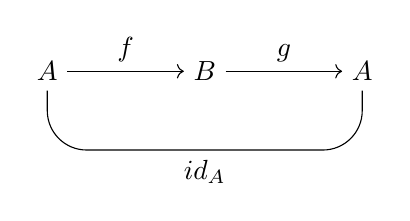
\begin{tikzpicture}[node distance=2cm]
		\node (B) at (0,0){$B$};
		\node[right of=B] (C){$A$};
		\node[left of=B] (A){$A$};
		\node[below of=B,node distance=1cm] (id){};
		\draw[->] (A)--(B) node[above,midway]{$f$};
		\draw[->] (B)--(C) node[above,midway]{$g$};
		\draw (id) node[below]{$id_A$};
		\draw[rounded corners=5mm] (A)|-(id.center)-|(C);
	\end{tikzpicture}
\end{document}